\documentclass[man, fleqn, noextraspace]{apa6}
\usepackage{lmodern}
\usepackage{amssymb,amsmath}
\usepackage{ifxetex,ifluatex}
\usepackage{fixltx2e} % provides \textsubscript
\ifnum 0\ifxetex 1\fi\ifluatex 1\fi=0 % if pdftex
  \usepackage[T1]{fontenc}
  \usepackage[utf8]{inputenc}
\else % if luatex or xelatex
  \ifxetex
    \usepackage{mathspec}
  \else
    \usepackage{fontspec}
  \fi
  \defaultfontfeatures{Ligatures=TeX,Scale=MatchLowercase}
\fi
% use upquote if available, for straight quotes in verbatim environments
\IfFileExists{upquote.sty}{\usepackage{upquote}}{}
% use microtype if available
\IfFileExists{microtype.sty}{%
\usepackage{microtype}
\UseMicrotypeSet[protrusion]{basicmath} % disable protrusion for tt fonts
}{}
\usepackage{hyperref}
\hypersetup{unicode=true,
            pdftitle={Differences in Stress Response by Ethnicity},
            pdfauthor={Ruby Cuellar, Ellen Huang, \& Angela Lee},
            pdfkeywords={sleep, stress, ethnicity},
            pdfborder={0 0 0},
            breaklinks=true}
\urlstyle{same}  % don't use monospace font for urls
\usepackage{graphicx,grffile}
\makeatletter
\def\maxwidth{\ifdim\Gin@nat@width>\linewidth\linewidth\else\Gin@nat@width\fi}
\def\maxheight{\ifdim\Gin@nat@height>\textheight\textheight\else\Gin@nat@height\fi}
\makeatother
% Scale images if necessary, so that they will not overflow the page
% margins by default, and it is still possible to overwrite the defaults
% using explicit options in \includegraphics[width, height, ...]{}
\setkeys{Gin}{width=\maxwidth,height=\maxheight,keepaspectratio}
\IfFileExists{parskip.sty}{%
\usepackage{parskip}
}{% else
\setlength{\parindent}{0pt}
\setlength{\parskip}{6pt plus 2pt minus 1pt}
}
\setlength{\emergencystretch}{3em}  % prevent overfull lines
\providecommand{\tightlist}{%
  \setlength{\itemsep}{0pt}\setlength{\parskip}{0pt}}
\setcounter{secnumdepth}{0}
% Redefines (sub)paragraphs to behave more like sections
\ifx\paragraph\undefined\else
\let\oldparagraph\paragraph
\renewcommand{\paragraph}[1]{\oldparagraph{#1}\mbox{}}
\fi
\ifx\subparagraph\undefined\else
\let\oldsubparagraph\subparagraph
\renewcommand{\subparagraph}[1]{\oldsubparagraph{#1}\mbox{}}
\fi

%%% Use protect on footnotes to avoid problems with footnotes in titles
\let\rmarkdownfootnote\footnote%
\def\footnote{\protect\rmarkdownfootnote}


  \title{Differences in Stress Response by Ethnicity}
    \author{Ruby Cuellar\textsuperscript{1}, Ellen Huang\textsuperscript{1}, \& Angela Lee\textsuperscript{1}}
    \date{}
  
\shorttitle{DIFFERENCESINSTRESSRESPONSE}
\affiliation{
\vspace{0.5cm}
\textsuperscript{1} University of Oregon}
\keywords{sleep, stress, ethnicity\newline\indent Word count: X}
\usepackage{csquotes}
\usepackage{upgreek}
\captionsetup{font=singlespacing,justification=justified}

\usepackage{longtable}
\usepackage{lscape}
\usepackage{multirow}
\usepackage{tabularx}
\usepackage[flushleft]{threeparttable}
\usepackage{threeparttablex}

\newenvironment{lltable}{\begin{landscape}\begin{center}\begin{ThreePartTable}}{\end{ThreePartTable}\end{center}\end{landscape}}

\makeatletter
\newcommand\LastLTentrywidth{1em}
\newlength\longtablewidth
\setlength{\longtablewidth}{1in}
\newcommand{\getlongtablewidth}{\begingroup \ifcsname LT@\roman{LT@tables}\endcsname \global\longtablewidth=0pt \renewcommand{\LT@entry}[2]{\global\advance\longtablewidth by ##2\relax\gdef\LastLTentrywidth{##2}}\@nameuse{LT@\roman{LT@tables}} \fi \endgroup}


\DeclareDelayedFloatFlavor{ThreePartTable}{table}
\DeclareDelayedFloatFlavor{lltable}{table}
\DeclareDelayedFloatFlavor*{longtable}{table}
\makeatletter
\renewcommand{\efloat@iwrite}[1]{\immediate\expandafter\protected@write\csname efloat@post#1\endcsname{}}
\makeatother
\raggedbottom
\setlength{\parskip}{0pt}

\authornote{

Correspondence concerning this article should be addressed to Ruby Cuellar, Department of Psychology, 1227 University of Oregon, Eugene, OR 97403. E-mail: \href{mailto:rcuellar@uoregon.edu}{\nolinkurl{rcuellar@uoregon.edu}}}

\abstract{
One or two sentences providing a \textbf{basic introduction} to the field, comprehensible to a scientist in any discipline.

Two to three sentences of \textbf{more detailed background}, comprehensible to scientists in related disciplines.

One sentence clearly stating the \textbf{general problem} being addressed by this particular study.

One sentence summarizing the main result (with the words ``\textbf{here we show}'' or their equivalent).

Two or three sentences explaining what the \textbf{main result} reveals in direct comparison to what was thought to be the case previously, or how the main result adds to previous knowledge.

One or two sentences to put the results into a more \textbf{general context}.

Two or three sentences to provide a \textbf{broader perspective}, readily comprehensible to a scientist in any discipline.


}

\begin{document}
\maketitle

\hypertarget{introduction}{%
\section{Introduction}\label{introduction}}

Sleep is essential for daily functioning, health, and optimal development. Disturbed or poor sleep has the potential to impair levels of stress the following day (Garde, Albertsen, Persson, Hansen, \& Rugulies, 2012), as well modulates numerous physiological processes, including stress response and recovery. Findings such as these suggest that adequate sleep plays an important role in how individuals respond to stress. High stress due to lack of sleep causes a dysregulation to the autonomic nervous system, specifically the sympathetic nervous system (SNS) (Mellman, Bell, Abu-Bader, \& Kobayashi, 2018). Hyperactivity of the SNS has been long recognized as a major risk of the relationship between stress and cardiovascular disease (Cohen, Janicki-Deverts, \& Miller, 2007). Contrary, the parasympathetic nervous system (PNS) regulates the SNS activity to bring the ANS back to homeostasis. Sleep is one mechanism by which PNS offsets SNS activity (Mellman et al., 2018). Consequently, insufficient sleep due to stress is a risk factor for a variety of physical and psychological problems, such as cardiovascular disease, obesity, diabetes, depression, and anxiety (Fuligni \& Hardway, 2006).

Adolescents are at high risk of insufficient sleep (Tsai \& Li, 2004), particularly as they transition into college (Doane, Gress-Smith, \& Breitenstein, 2015; Sladek \& Doane, 2015). Many university students meet the requirements for partial sleep deprivation (e.g.~less than 5 hours of sleep in a 24-hour period) and delayed sleep phase syndromes (difficulty falling asleep and waking up) (Galambos, Dalton, \& Maggs, 2009). The complex demands on college students, coupled with the risk created by insufficient sleep, makes understanding the link between sleep and stress response and recovery a priority. Additionally, college is an opportune time for interventions, which set the stage for long-term behavioral health.

The United States population and college student body is growing increasingly diverse. Latinos are the largest ethnic minority group in the U.S, with Mexican Americans being the largest subgroup, and are expected to comprise approximately 30\% of the population by 2050. Latinos face health disparities compared to non-Latino Whites, such as higher rates of cardiovascular heart disease (Hunt et al., 2003), obesity, and diabetes, all three which have been linked to sleep problems in other populations (Howrey, Peek, Raji, Ray, \& Ottenbacher, 2012). Additionally, co-existing sleep problems such as sleep apnea or sleep deprivation could also impact the management of diabetes, obesity, and other sleep related conditions. This data suggests a potential bi-directional effect between sleep and well-being and highlights the importance of understanding mechanisms that might contribute to poor health, such as insufficient sleep and impaired stress response and recovery.

There is a small body of evidence that Latinos are at-risk of insufficient sleep (Jean-Louis, Kripke, Ancoli-Israel, Klauber, \& Sepulveda, 2000; Loredo et al., 2010). Some data suggests that the prevalence of sleep problems and predictors of sleep duration are different in Latinos versus Whites. Such differences include differences in sleep architecture, such that Latino children experience less deep sleep than White children (Loredo et al., 2010). Additionally, Latinos have higher risk of insomnia and hyperinsomnia, and differences in environmental determinants; specifically Latino children are more likely to live in environments that disturb their sleep. Much of the limitations in knowledge stem from under-representation of Latinos in sleep research (Jean-Louis et al., 2000; Knutson, 2010; Krueger \& Friedman, 2009; Pedraza, Al Snih, Ottenbacher, Markides, \& Raji, 2012). Importantly, no studies have examined the link between sleep and stress response or recovery among Latino college students in a prospective, quasi-experimental study.

This study aims to elucidate the role of Latino ethnicity in the link between sleep and stress response and recovery among college students by comparing equivalent size groups of Latino and non-Latino white young adults. Identifying variation in the link between sleep and stress response and recovery by ethnicity would stimulate the development of culturally sensitive prevention and intervention programs. It is hypothesized that being Latino will influence the strength of the relationship between sleep duration and quality and stress response and recovery. Specifically, it is expected that Latinos will experience greater stress response and diminished stress recovery compared to Whites. Support for this hypothesis would provide a framework for addressing health disparities.

\hypertarget{methods}{%
\section{Methods}\label{methods}}

\hypertarget{design}{%
\subsection{Design}\label{design}}

This is a quasi-experimental study in which equivalent groups of Latino and non-Latino white college students were exposed to a stress manipulation to observe their physiological stress response and recovery. Self-reported sleep was measured prospectively for ten days leading up to the stress induction.

\hypertarget{participants}{%
\subsection{Participants}\label{participants}}

A sample of 133 undergraduate students (53\% Mexican American, 47\% Whites) were recruited from a Human Participant Pool (HPP) or summer classes at a university in Southern California. Inclusion criteria required participants to be enrolled college students, be 18-24 years old, be proficient in English and identify themselves as being Mexican American or White. The requirement of being Mexican American was to provide homogeneity within the diverse Latin American culture; Mexican American was chosen because it is the largest country of origin among U.S. Latinos (Loredo et al., 2010). Participants who reported any medical condition that could be exacerbated from stress, reported having an extreme fear of public speaking, had a current psychiatric diagnosis related to stress, or an inability to cope with stress were excluded from the study.

\hypertarget{measures}{%
\subsection{Measures}\label{measures}}

\hypertarget{descriptive-measures}{%
\subsubsection{Descriptive Measures}\label{descriptive-measures}}

\emph{Demographics.} Participants were asked demographic questions about race/ethnicity, generation status, gender, and age.

\hypertarget{sleep-characteristics}{%
\subsubsection{Sleep Characteristics}\label{sleep-characteristics}}

\emph{Daily Diary.} Sleep patterns were monitored with an online sleep diary. Students were instructed to complete a three-minute survey every night before bed for ten consecutive nights. The daily diaries consisted of questions pertaining to the prior night's sleep (adapted from (Fuligni, Tsai, Krull, \& Gonzales, 2015)). The diaries assessed the participants sleep duration and sleep quality. A mean for both sleep domains was calculated from the daily diary surveys.

\hypertarget{stress-induction}{%
\subsubsection{Stress Induction}\label{stress-induction}}

\emph{Trier Social Stress Task.} The Trier Social Stress Test (TSST), adapted by Yim, Quas, Rush, Granger, and Skoluda (2015) was used to induce stress. During the TSST, the participant entered a room where one male and one female judge were waiting. The participants were instructed to deliver a 5-minute speech, followed by mental arithmetic in front of the judges while being videotaped. If at any moment they stopped, they were instructed to continue with the task until the five minutes were up (only two reminders were allowed). If they stopped again or remained silent for 15 seconds, the judge would instruct them to continue standing for the remainder of the time.

\hypertarget{stress-response-and-recovery.}{%
\subsubsection{Stress Response and Recovery.}\label{stress-response-and-recovery.}}

\emph{Autonomic stress response.} The study assessed the participants' autonomic response to stress by measuring heart rate, specifically mean beats per minute (BPM) and heart rate variability (HRV), using Biopac wireless Electrocardiogram (ECG) equipment and Bionomadix software. Participants were connected to the Biopac system using wireless Electrocardiogram (ECG) equipment five minutes before the initiation of the TSST in order to get a baseline measure and remained connected until the completion of the study. Three mean heart rate values were extracted for each participant for each measure of heart rate. In other words, 5 minutes were extracted from baseline (T1), 15 minutes during the TSST (T2), and 35-min during recovery (T3) for both BPM and HRV. Stress reactivity corresponds to the change score from baseline to TSST (T1 and T2), while stress recovery corresponds to change scores from TSST and recovery (T2 and T3).

\hypertarget{procedure}{%
\subsection{Procedure}\label{procedure}}

The present study consisted of two sessions with a ten-day, daily assessment in-between the sessions. During Session 1, participants provided consent to the study. They were then screened to see if they met the criteria required to participate. Qualified participants were asked to fill out their demographic information and given instructions for the at home portion that involved the daily diaries. Lastly, participants were scheduled for Session 2. Session 2 was scheduled about two weeks after the initial visit. During the at home portion of this study, participants were instructed to fill out an online survey about their daily sleeping habits before bed, every night, for ten consecutive days. Participants automatically received an email at 6 am the following morning reminding them to complete the diary in case they had forgotten. Participants were told to ignore the second email if the diary had been completed the night before. Session 2 was the final stage of the study, upon arrival participants were introduced to the task environment, and hooked up to the wireless ECG equipment. Participants were asked to relax and breathe normally for five minutes while baseline heart rate was measured. Following the baseline, participants were briefed on the speech task. They were given three minutes to prepare a 5-minute mock interview to deliver in front of a panel that they believed were judging their performance. Following the speech, participants were instructed to perform some basic mental arithmetic -- serial subtraction -- for 5 minutes. At the conclusion of both tasks, the 35-minute recovery period began. Participants were given a questionnaire packet to complete as well as an eleventh daily diary to control for the previous night's sleep. Upon completing the questionnaires, participants were invited to read neutral material and relax in the pre-task room for the remainder of the time. At the conclusion of the 35 minutes, the participants were unhooked from the Biopac equipment, were debriefed on the study, and supplied a referral for counseling services at the university.

\hypertarget{analytic-approach}{%
\subsection{Analytic Approach}\label{analytic-approach}}

Following data collection and data entry, all data was checked in order to assess for normality, skewness, kurtosis, missing data, and outliers. Winsorizing was used to correct for normality and to address outliers. Given the high attrition rate of this study, 133 participants completed daily diaries; however, not all participants completed the second session. Due to this and uninterruptible heart rate data, the final sample was reduced to 107. In order to account for the participants' sleep the night prior to the stressors, an eleventh dairy was controlled for. However, this block was removed from the analysis because the eleventh diary did not significantly contribute to the overall model. Participants' stress reactivity (changes in heart rate and heart rate variability) was regressed onto their self-reported measures of sleep duration and ethnicity and the interaction between them. We used R Version 3.6.1 (R Core Team, 2019) for all our analyses.

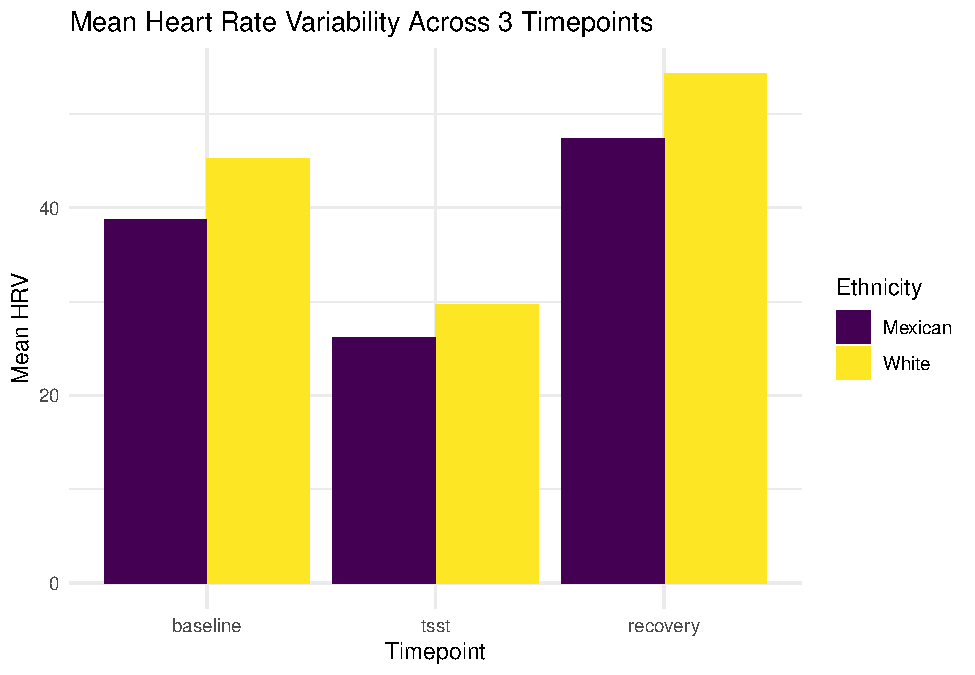
\includegraphics{PAPAJA_Final_class_project_files/figure-latex/visualization-1.pdf} 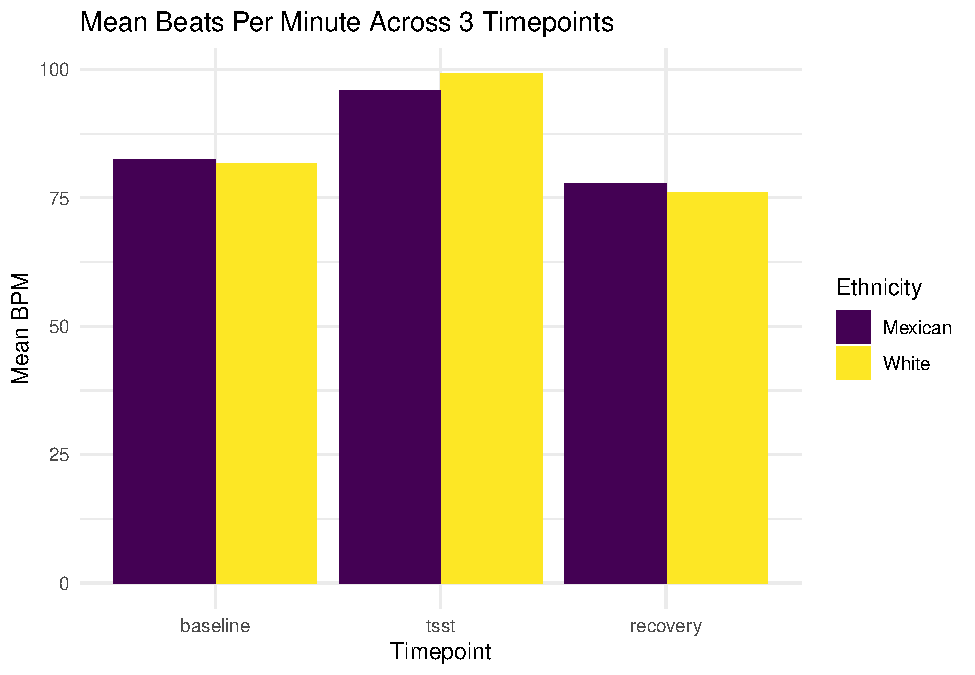
\includegraphics{PAPAJA_Final_class_project_files/figure-latex/visualization-2.pdf}

\hypertarget{results}{%
\section{Results}\label{results}}

Participant characteristics are displayed in Table 1. Consistent with the demographics of the university, participants were predominantly female (77\%). When analyzing heart rate, both BPM and HRV demonstrated normal stress response. Two one-way analysis of variances (ANOVAs) were conducted to determine difference among the three time points in BPM and HRV. The first ANOVA demonstrated significant variation among time points in HRV F(2,3) = 15.87, p = .03. A post hoc Tukey test revealed that the difference lies between TSST (M = 27.9, SD = 14.8) and recovery (M = 50.8, SD = 29.8). The second ANOVA test also yielded significant variation among the three time points in BPM F(2,3) = 100.7, p = .002, a post hoc Tukey test revealed the differences between time points were at Baseline (M = 82.1, SD = 13.3) and TSST (M = 97.6, SD = 15.7) and TSST (M = 97.6, SD = 15.7) and recovery (M = 76.9, SD = 10.6).

\begin{tabular}{r|r|r|r|r|r}
\hline
mean\_hrv\_baseline & mean\_hrv\_tsst & mean\_hrv\_recovert & mean\_bpm\_baseline & mean\_bpm\_tsst & mean\_bpm\_recovery\\
\hline
41.96165 & 27.91561 & 50.39149 & 82.08148 & 97.55962 & 76.27081\\
\hline
\end{tabular}

When examining ethnicity as a moderator for the relationship between sleep domains (quality and duration) and stress response (reactivity and recovery) for both measures of heart rate (BPM and HRV), eight moderation analyses were conducted. Results demonstrated no significant interactions between sleep and ethnicity for any moderation model. However, main effects of ethnicity were found for both sleep domains and both stress reactivity and stress recovery when measured by mean BPM. Therefore, the interaction terms were dropped and simple regression was conducted to examine the association between ethnicity and stress reactivity and recovery. Regression analysis results indicate that White participants were more likely to experience an increase in heart rate during stressor, F(1, 113) = 4.56, p = 0.03, R2 = .04, and more likely to recover faster from the stressor, F(1, 113) = 7.11, p = 0.009, R2 = .06, than Mexican American participants.

\hypertarget{discussion}{%
\section{Discussion}\label{discussion}}

\newpage

\hypertarget{references}{%
\section{References}\label{references}}

\begingroup
\setlength{\parindent}{-0.5in}
\setlength{\leftskip}{0.5in}

\hypertarget{refs}{}
\leavevmode\hypertarget{ref-cohen2007_psych}{}%
Cohen, S., Janicki-Deverts, D., \& Miller, G. E. (2007). Psychological stress and disease. \emph{Jama}, \emph{298}(14), 1685--1687.

\leavevmode\hypertarget{ref-doane2015multi}{}%
Doane, L. D., Gress-Smith, J. L., \& Breitenstein, R. S. (2015). Multi-method assessments of sleep over the transition to college and the associations with depression and anxiety symptoms. \emph{Journal of Youth and Adolescence}, \emph{44}(2), 389--404.

\leavevmode\hypertarget{ref-fuligni2006daily}{}%
Fuligni, A. J., \& Hardway, C. (2006). Daily variation in adolescents' sleep, activities, and psychological well-being. \emph{Journal of Research on Adolescence}, \emph{16}(3), 353--378.

\leavevmode\hypertarget{ref-fuligni2015daily}{}%
Fuligni, A. J., Tsai, K. M., Krull, J. L., \& Gonzales, N. A. (2015). Daily concordance between parent and adolescent sleep habits. \emph{Journal of Adolescent Health}, \emph{56}(2), 244--250.

\leavevmode\hypertarget{ref-galambos2009losing}{}%
Galambos, N. L., Dalton, A. L., \& Maggs, J. L. (2009). Losing sleep over it: Daily variation in sleep quantity and quality in canadian students' first semester of university. \emph{Journal of Research on Adolescence}, \emph{19}(4), 741--761.

\leavevmode\hypertarget{ref-garde_2012_bi}{}%
Garde, A. H., Albertsen, K., Persson, R., Hansen, Å. M., \& Rugulies, R. (2012). Bi-directional associations between psychological arousal, cortisol, and sleep. \emph{Behavioral Sleep Medicine}, \emph{10}(1), 28--40.

\leavevmode\hypertarget{ref-howrey2012self}{}%
Howrey, B. T., Peek, M. K., Raji, M. A., Ray, L. A., \& Ottenbacher, K. J. (2012). Self-reported sleep characteristics and mortality in older adults of mexican origin: Results from the h ispanic e stablished p opulation for the e pidemiologic s tudy of the e lderly. \emph{Journal of the American Geriatrics Society}, \emph{60}(10), 1906--1911.

\leavevmode\hypertarget{ref-hunt2003all}{}%
Hunt, K. J., Resendez, R. G., Williams, K., Haffner, S. M., Stern, M. P., \& Hazuda, H. P. (2003). All-cause and cardiovascular mortality among mexican-american and non-hispanic white older participants in the san antonio heart study---evidence against the ``hispanic paradox''. \emph{American Journal of Epidemiology}, \emph{158}(11), 1048--1057.

\leavevmode\hypertarget{ref-jean2000sleep}{}%
Jean-Louis, G., Kripke, D. F., Ancoli-Israel, S., Klauber, M. R., \& Sepulveda, R. S. (2000). Sleep duration, illumination, and activity patterns in a population sample: Effects of gender and ethnicity. \emph{Biological Psychiatry}, \emph{47}(10), 921--927.

\leavevmode\hypertarget{ref-knutson2010sleep}{}%
Knutson, K. L. (2010). Sleep duration and cardiometabolic risk: A review of the epidemiologic evidence. \emph{Best Practice \& Research Clinical Endocrinology \& Metabolism}, \emph{24}(5), 731--743.

\leavevmode\hypertarget{ref-krueger2009sleep}{}%
Krueger, P. M., \& Friedman, E. M. (2009). Sleep duration in the united states: A cross-sectional population-based study. \emph{American Journal of Epidemiology}, \emph{169}(9), 1052--1063.

\leavevmode\hypertarget{ref-loredo2010sleep}{}%
Loredo, J. S., Soler, X., Bardwell, W., Ancoli-Israel, S., Dimsdale, J. E., \& Palinkas, L. A. (2010). Sleep health in us hispanic population. \emph{Sleep}, \emph{33}(7), 962--967.

\leavevmode\hypertarget{ref-mellman_2018_SNS}{}%
Mellman, T. A., Bell, K. A., Abu-Bader, S. H., \& Kobayashi, I. (2018). Neighborhood stress and autonomic nervous system activity during sleep. \emph{Sleep}, \emph{41}(6), zsy059.

\leavevmode\hypertarget{ref-pedraza2012sleep}{}%
Pedraza, S., Al Snih, S., Ottenbacher, K. J., Markides, K. S., \& Raji, M. A. (2012). Sleep quality and sleep problems in mexican americans aged 75 and older. \emph{Aging Clinical and Experimental Research}, \emph{24}(4), 391--397.

\leavevmode\hypertarget{ref-R-base}{}%
R Core Team. (2019). \emph{R: A language and environment for statistical computing}. Vienna, Austria: R Foundation for Statistical Computing. Retrieved from \url{https://www.R-project.org/}

\leavevmode\hypertarget{ref-sladek2015daily}{}%
Sladek, M. R., \& Doane, L. D. (2015). Daily diary reports of social connection, objective sleep, and the cortisol awakening response during adolescents' first year of college. \emph{Journal of Youth and Adolescence}, \emph{44}(2), 298--316.

\leavevmode\hypertarget{ref-tsai2004sleep}{}%
Tsai, L.-L., \& Li, S.-P. (2004). Sleep patterns in college students: Gender and grade differences. \emph{Journal of Psychosomatic Research}, \emph{56}(2), 231--237.

\leavevmode\hypertarget{ref-yim2015experimental}{}%
Yim, I. S., Quas, J. A., Rush, E. B., Granger, D. A., \& Skoluda, N. (2015). Experimental manipulation of the trier social stress test-modified (tsst-m) to vary arousal across development. \emph{Psychoneuroendocrinology}, \emph{57}, 61--71.

\endgroup


\end{document}
